 \chapter{Appendix}
    \section{Graphs}
     \subsection{Matrix-based Graph Representations}\label{mbr}
        \subsubsection*{Adjacency Matrix}
            An adjacency matrix of a graph $G$ is a $|V|\times|V|$ matrix where a non-zero entry corresponds to an edge with the weight being the value of that entry. 
            Let $A \in |V|\times|V|, \ u, v \in \{0, \dots, |V| - 1\}$ and $w_{u,v}$ the weight of the edge $e = (u,v) \in E$ then
            \[ a_{uv} = \begin{cases}
                        w_{u,v} & \text{if } (u,v) \in E \\
                        0 & \text{otherwise}
                        \end{cases}
            \]
            Additionally, to model non-consecutive indices, one needs to store a mapping from the actual vertex index to the one used in the matrix --- usually represented by a 2D array. 
            It is also important to note that adjacency matrix representations cannot represent multi-graphs without further modification.
            The space complexity of an adjacency matrix is thus $\mathcal{O}(|V|^2 + |V|)$.
            \begin{figure}[htp]
            \begin{center}
            \begin{minted}[fontsize=\footnotesize]{bash}
                0 1 2 3 4 5 6 7
                0 1 2 3 4 7 9 10
            \end{minted}
            \begin{minted}{bash}
                0 1 0  0 0 0 0 0
                2 0 1  1 0 0 0 0
                0 0 0 -1 0 0 0 0
                0 0 0  0 1 0 0 0
                0 5 0  0 0 0 0 0
                0 0 0  0 0 0 3 0
                0 0 0  0 0 0 0 0
                0 0 0  0 0 0 0 0
            \end{minted}
            \end{center}
            \caption{An example of the adjacency matrix representation of a graph.}
            \label{adm}
            \end{figure} 
            The number of nodes can be retrieved in $\mathcal{O}(1)$, as it is simply the size of the stored mapping.
            For the number of edges, one needs to iterate over all matrix elements and count the non-zero entries, which requires one to touch $\mathcal{O}(|V|^2)$ elements.
            Finding a vertex is just an array lookup, thus $\mathcal{O}(1)$.
            Insertion requires adding one row and one column to the matrix and one entry to the mapping. 
            This includes reallocating the matrix, which is non-deterministic and independent of the matrix size. However, it also requires copying all elements to the new matrix, such that we can estimate the overall asymptotic runtime of $\mathcal{O}(|V|^2)$.
            Deleting a vertex is similar. Either one leaves a gap that may be used on subsequent insertions and marks the true id in the mapping as deleted, which would be an $\mathcal{O}(1)$ operation. 
            Alternatively, one could immediately reallocate the matrix to free the extra row and column and the extra field in the mapping. 
            This would again be non-deterministic but can again be estimated by copying the elements from the former matrix $\mathcal{O}(|V-1|^2) = \mathcal{O}(|V|^2)$.
            For edges, the basic operations find, insert and remove can be executed in constant runtime, i.e., $\mathcal{O}(1)$, as simple array access.
            Deciding whether two vertices are adjacent requires just reading what is in the particular array at the index of the two nodes, $\mathcal{O}(1)$ runtime.
            Finally, finding the neighborhood $N_v$ of a vertex requires a scan of a row and a column again, i.e., an asymptotic runtime of $\mathcal{O}(2|V|)$. For the incoming and outgoing sets of a vertex, one needs to access only a row or a column resulting in $\mathcal{O}(|V|)$ steps per operation.
            An example of this data structure is shown in Listing~\ref{adm}.

        \subsubsection*{Incidence Matrix}
            An incidence matrix of a graph $G$ is an $|V| \times |E|$ matrix, where each column corresponds to an edge. 
            Each entry in a column is either the positive weight if the node is the target of the edge or the negative weight if the node is the edge's source. Self-loops require a slight extension of this syntax because one node would be both source and target such that the entry is zero. One option is just to put the weight as an entry of the node.  Another problem is that incidence matrices can not represent negative weights without further extensions.        
            Let $u,v \in \{0, |V|-1\}, j \in \{0, |E|-1\}, A \in |V| \times |E|$ and $a_{v,j}$ the entry at row $v$ and column $j$ of $A$. Let further $w_j$ be the weight of the edge $e_j = (u,v) \in E$. Then 
            \[         a_{vj} = \begin{cases}
                        -w_{v,u} & \text{if } e_j = (v,u) \in E \\
                        w_{u,v} & \text{if } e_j = (u,v) \in E \\
                        0 & \text{otherwise}
                        \end{cases}
            \]
            
            As with adjacency matrices, to represent non-consecutive indices, we need to store a mapping from the true node indices to the ones used in the matrix.
            The space requirements are thus $\mathcal{O}(|V| \cdot |E| + |V|) = \mathcal{O}(|V| \cdot |E|)$.
            
            \begin{figure}[htp]
         \begin{center}
         \begin{minted}[fontsize=\footnotesize]{bash}
            0 1 2 3 4 5 6 7
            0 1 2 3 4 7 9 10
          \end{minted}
          \begin{minted}{bash}
            -1  2  0  0    0   0  0
            1  -2 -1 -(-1) 0   5  0
            0   0  1  0    0   0  0
            0   0  0  (-1) 1   0  0
            0   0  0  0    1  -5  0
            0   0  0  0    0   0  0
            0   0  0  0    0   0 -3
            0   0  0  0    0   0  3
          \end{minted}
         \end{center}
         \caption{An example of the incidence matrix representation of a graph.}
         \label{incm}
        \end{figure}
            
            The number of nodes can be retrieved in $\mathcal{O}(1)$, as it is simply the size of the stored mapping.
            The number of edges can also be retrieved in $\mathcal{O}(1)$ as it is the second dimension of the matrix.
            Finding a vertex is just an array lookup, thus $\mathcal{O}(1)$.
            Insertion requires adding one row and one column to the matrix and one entry to the mapping, as with adjacency lists. 
            Thus the complexity is again the cost of copying the whole matrix $\mathcal{O}(|V| \cdot |E|)$. 
            The same is true for deleting a vertex.         
            To find an edge, one needs to scan one row of either the source or the edge's target node, which requires $\mathcal{O}(|E|)$ steps.
            Insertion and removal of edges correspond to the case of vertices.
            One would need to reallocate the matrix and copy all elements resulting in an asymptotic runtime complexity of $\mathcal{O}(|V| \cdot |E|)$. 
            Deciding whether two vertices are adjacent requires reading one row and checking for each non-zero element if the entry in the other nodes row is also non-zero, which has $\mathcal{O}(|E|)$ runtime.        
            Finally, finding the neighborhood $N_v$ of a vertex requires a scan of a row again and checking all non-zero entry columns for the neighbor, i.e., an asymptotic runtime of $\mathcal{O}(|E|)$. 
            For the incoming and outgoing sets, the procedure is almost the same. 
            The difference is that only positive or negative non-zero columns --- depending on whether the incoming or outgoing neighbors shall be returned -- have to be checked.
            An example of this data structure is shown in Listing~\ref{incm}.
        

        
    \subsection{Additional Graph Partitioning Algorithms}
        \subsubsection*{Kernighan-Lin Algorithm}\label{kla}
            The Kernighan-Lin (KL) algorithm~\autocite{kl} was invented by Brain Kernighan --- one of the creators of Unix and co-author of the de facto standard book ''The C Programming Language`` and  Shen Lin.
            It was developed and is used for laying out digital circuits on a chip. 
            It is also used by many other more complex graph partitioning algorithms as the multilevel partitioning algorithm implementation of Karypis and Kumar~\autocite{karypis} described in the next part.
            
            \begin{figure}[htp]
                \begin{center}
                    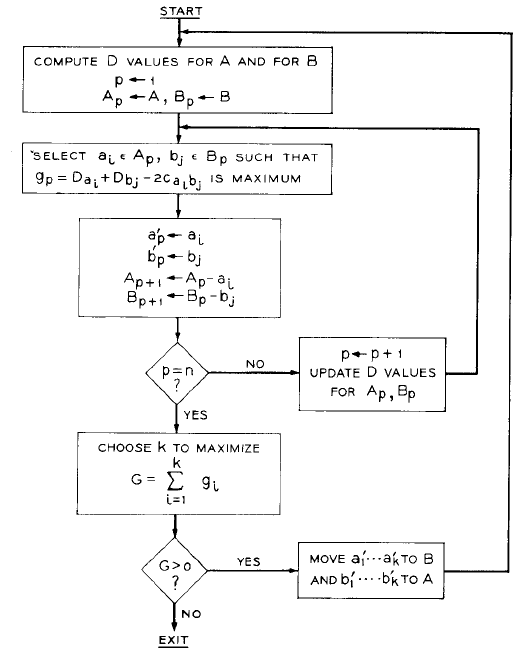
\includegraphics[keepaspectratio,width=0.55\textwidth]{img/03-graphs/kl.png}
                \end{center}
                \caption{A flow diagram of the KL algorithm~\autocite{kl}.} 
                \label{kl-fig}
            \end{figure}
                
            The KL algorithm, in its most basic form, finds a minimal cut of the graph into two disjoint partitions of the same size. 
            It assumes an undirected graph and is extended to unequally sized partitions and $k$-way partitioning. 
            To decide which node has to be in which partition a cost function $D(v)$ is used. 
            Let $v  \in V_i$ and $i \neq j$. $I(v)$ is called the internal cost of $v$, $E(v)$ is called the external cost of $v$ with
            \[ I(v) = \sum_{u \in V_i} w_{(u, v)} \]
            \[ E(v) = \sum_{s \in V_i} w_{(s, v)} \]
            \[   D(v) = E(v) - I(V)   \]
            The internal cost is thus the sum of all edge weights within a partition incident to a specific vertex, while the external cost is the sum of all edge weights to vertices in the other partition for a specific vertex. 
            The overall cost function is just the difference between external and internal cost.
            The gain of exchanging two vertices between partitions is proven~\autocite{kl} to be --- with $v \in V_i, s \in V_j, i \neq j$
            \[ g = D_v + D_s - 2 w_{(v,s)} \]
            
            The most basic form works as follows.
            \begin{enumerate}
                \item Split the set of vertices into two partitions arbitrarily.
                \item $\forall v \in V$ compute $D(v)$.
                \item Select $v \in V_i, s \in V_j, i \neq j$ such that $g$ is maximal. Exclude them from their partitions.
                \item Update the $D$ values for all remaining nodes in both partitions using 
                \[ u \in V_i \setminus {v}: D'(u) = D(u) + 2 w_{(u, v)} - 2 w_{(u, s)} \]
                \[ x \in V_j \setminus {s}: D'(x) = D(x) + 2 w_{(x, s)} - 2 w_{(s, v)} \]
                \item Go to 3 until the partitions are empty.
                \item choose $k$ to maximize 
                \[ G = \sum^k_{i = 0} g_i \]
                \item If $G > 0$ apply the swaps and go to 2. Else terminate
            \end{enumerate}
            The steps are summarized in the flow diagram in Figure~\ref{kl-fig}.
            Regarding the extensions, an improvement schema is provided to avoid local optima.
            Apply the algorithm to the so-created partitions and union the partitions alternatingly (i.e., $A_1 \cup B_2, A_2 \cup B_1$) and use these partitions as initialization of the algorithm.
            To create partitions of unequal size with $n_1$ being the minimal desired partition size and $n_2$ the maximal desired partition size, add dummy vertices, such that we have $2n_2$ vertices in total and restrict the number of changes that are allowed to $n_1$.
            For partitioning the graph into $k$-partitions, one needs to split the initial set of vertices into $k$ partitions. 
            Then apply the 2-way partitioning algorithm pairwise to all partitions until convergence.
            
            One pass of the basic form of the algorithm is in $\mathcal{O}(|V|^2 \cdot \log(|V|))$. The $k$-way partitioning algorithm requires per iteration $\binom{k}{2} = \frac{k (k - 1)}{2}$ executions of the algorithm, thus $\mathcal{O}(k^2 \cdot |V|^2 \cdot \log(|V|)$ in total, assuming that the number of iterations is small as shown empirically by the authors~\autocite{kl}. Further improvements were developed in the years after publication, for example, a linear-time implementation applicable to hypergraphs by Fiduccia and Mattheyses~\autocite{fm}.

        \subsubsection*{Leiden Method}
            The Leiden method~\autocite{traag2019louvain} is an extension of the louvain method.
            It changes and extends the louvain method in three aspects.
            \begin{enumerate}
                \item It changes the quality function introducing an additional resolution parameter.
                \item It incorporates improvements by other authors on how nodes are moved between partitions~\autocite{movd,movc,movb,mova}.
                \item It adds a refinement stage after the contraction of the graph has converged.
            \end{enumerate}
            The quality function that is used by the Leiden method overcomes the problem of the resolution limit~\autocite{traag2011narrow, fortunato2007resolution}.
            It is called the Constant Potts Model~\autocite{potts1952some, traag2011narrow} and defined by 
            \[ CPM = \sum_{u,v \in V}(w_{(u,v)} + \gamma) \delta(u, v) \]
            where $G$ is a graph, $P$ is a partitioning of $G$, $w_{(u,v)}$ is the edge weight between $u$ and $v$, and $\gamma$ is the resolution parameter. 
            Intuitively it controls the coarseness of the partition and replaces the term $\frac{w_u w_v}{2m}$.
            A partition is formed, if its density is at least $\gamma$ and the density between partitions should be less than $\gamma$~\autocite{traag2019louvain}.
            
            \begin{figure}[htp]
                \begin{center}
                    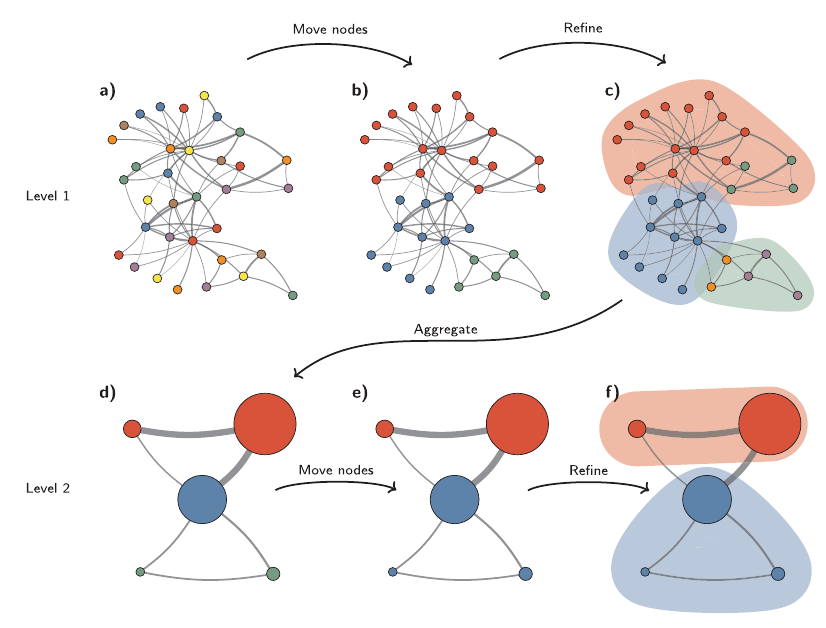
\includegraphics[keepaspectratio,width=0.6\textwidth]{img/03-graphs/leiden.png}
                \end{center}
                \caption{The steps that the leiden algorithm executes~\autocite{traag2019louvain}.} 
                \label{leiden-fig}
            \end{figure}
            
            The node movement is changed in a couple of ways.
            The Leiden algorithm keeps track of which neighborhoods changed and only visits these nodes again, in contrast to Louvain, which keeps iterating all nodes\autocite{movb, movc}.
            Initially, it adds all nodes to a queue, removes the first one, and adds the node's neighborhood to the queue only if it was moved.
            
            The refinement stage is added after moving nodes between communities and before aggregating the communities into a new graph.
            Starting with the partitioning $P$, the algorithm derives a refined partitioning $P_{\text{ref}}$.
            First, all nodes are again initialized as an own singleton community. 
            Now nodes which are in their own community $C^i_{\text{ref}}$ can again be merged with into another community $C^j_{\text{ref}}$, but this time only with those from the same community in the previous partitioning $C \in P$. 
            In essence, it forms from a given partitioning a finer-grained partitioning within the communities.
            Additionally, not the merge with the highest increase in the quality function is chosen, but the choice is made randomly with a higher probability for better quality values to avoid getting stuck in local optima~\autocite{mova}.
            
            Empirically, the Leiden algorithm converges faster with a higher modularity score, with appropriate values for $\gamma$. A good value to start is $\gamma = \frac{1}{2}$, which results in an approximation of the Louvain algorithm's quality function --- the modularity of Newman and Girvan~\autocite{girvan2002community}.
\newpage
\section{Database Architecture}\label{db-arch}
    The reason why we use databases is twofold:
    First, every computer is equipped with different kinds of memory, which differ in size, capacity, speed, and price per byte. 
    This induces the so-called memory hierarchy, the principle that few fast, expensive, low capacity memory is used close to the central processing unit, which gets layerwise augmented with increasingly slower, less expensive, higher capacity memory. 
    The last layer, which has the highest capacity, defines the overall capacity, while the smallest one is crucial for performance.
    Thus what is shown as secondary storage in Figure~\ref{mem-hier} is orders of magnitude slower in both latency and throughput.
    Nevertheless, it is also able to store orders of magnitude more data. 
    \begin{figure}[htp]
        \begin{center}
        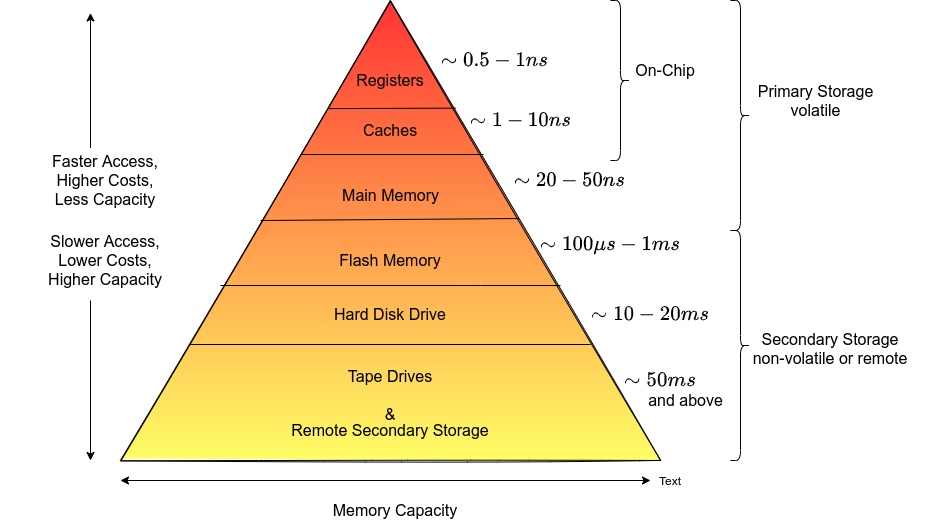
\includegraphics[keepaspectratio,width=0.8\textwidth]{img/04-databases/mem-hierarch.png}
        \end{center}
        \caption{The memory hierarchy used in today's computing systems.} 
        \label{mem-hier}
    \end{figure}
    To mitigate the effects of this, the accesses between primary and secondary memory need to be handled very carefully for data-intensive --- also called IO bound --- applications.
    Second, the operating system (OS) handles the first reason. 
    However, application-specific payloads enable further optimizations when it comes to how data is stored and accessed.
    Put differently, the operating system cannot infer certain information, as it does not constrain how data is stored, and as it does not profile in what patterns data is referenced or queried.
    Databases take care of these issues by different mechanisms, which will be lined out from a high-level perspective to understand how a database works on its architectural lower levels.
    Put differently, we are not going to discuss query processing, transactions, concurrency-related components, and recovery facilities.
    Most of the information below is outlined comprehensively in~\autocite{ramakrishnan2000database, silberschatz1997database}
    
    Let us consider the high-level architecture of a general database management system as shown in Figure~\ref{dbms_arch} --- with a focus on the storage and access elements.

    \begin{figure}[htp]
    \begin{center}
    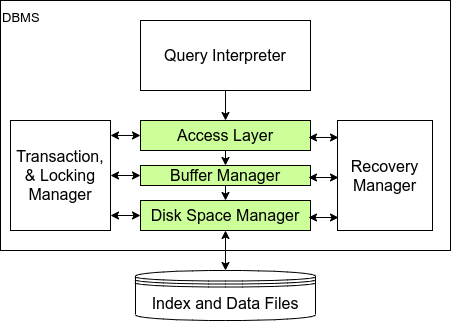
\includegraphics[keepaspectratio,width=.5\textwidth]{img/04-databases/RDBMS.png}
    \end{center}
    \caption{The typical structure of a relational database management system~\autocite{ramakrishnan2000database}.}
    \label{dbms_arch}
    \end{figure}

    The disk space manager, sometimes also called storage manager, handles de-/allocations, reads \& writes, and provides the concept of a block: One or many physical disk blocks are grouped to a logical disk block.
    These logical disk blocks are again grouped and brought into main memory (RAM) --- these groups are called a page.
    Optimally both a disk block and a page are of the same size or at least a multiple of each other. 
    Further, the database needs to keep track of free blocks in the file: 
    A linked list or a directory must record free blocks, and some structure needs to keep track of the free slots either globally or per block. 
    Data locality is a concept that we examine closely in an extra chapter later on.
    To summarize, the two most important objectives of a storage manager are to
    \begin{enumerate} 
     \item take care of (de-)allocations of disk space,
     \item abstract storing data on a physical device using the operating system: Files, split into logical disk blocks, accessed using OS facilities, and
     \item provide data structures in order to maintain records within a file, blocks.
    \end{enumerate}
    
    A buffer manager is used to mediate between external storage and main memory. 
    It provides the concept of a page and maintains a designated pre-allocated area of main memory --- called the buffer pool --- to load, cache, and evict pages into or from main memory~\autocite{ramakrishnan2000database}.
    A conceptual illustration of this is shown in \ref{buf-man}.
    Its objective is to minimize the number of disk reads to be executed by caching, pre-fetching, and the usage of suitable replacement policies. 
    It also needs to take care of allocating a certain fraction of pages to each transaction.

    \begin{figure}[htp]\label{dbms_memory}
        \begin{center}
        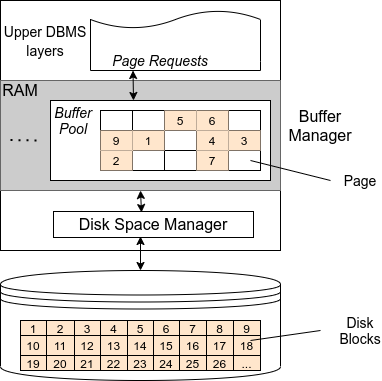
\includegraphics[keepaspectratio,height=0.4\textheight,width=0.5\textwidth]{img/04-databases/RDBMS_memory_view.png}
        \end{center}
        \caption{A visualization of the interaction of a database with memory~\autocite{ramakrishnan2000database}.}
        \label{buf-man}
    \end{figure}

    The final component crucial to the storage of data of a database management system is the file and record layout, along with possible index structures --- also called the access layer. 
    To store data, a DBMS may either use one single or multiple files to maintain records. 

    A file consists of a set of blocks split into slots.
    A slot stores one record, with each record containing a set of fields.
    Records can be layout in row- or column-major order.
    That is, one can store sequences of tuples or sequences of fields.
    The former is beneficial if many updates, insert, or delete operations are committed to the database, while the latter optimizes the performance when scans and aggregations are the most typical queries to the system.
    Records may be of fixed or of variable size, depending on the types of their fields. 
    Another option is to store the records' structure along with pointers to the values of their fields in one file and the actual values in one or multiple separate files. 
    Also, distinct types of tables can be stored in different files. 
    For example, entities and relations can be stored in different files with references to each other, thus enabling the layout of these two to be specialized to their structure and usage in queries.

    Files may either organize their records in random order (heap file), sorted, or using a hash function on one or more fields. 
    These approaches have upsides and downsides when it comes to scans, searches, insertions, deletions, and updates. 

    To mitigate the effect of selecting one file organization or another, one record organization or another, the concept of an index has been introduced. 
    Indexes are auxiliary structures to speed up certain operations or queries that depend on one field. 
    Indexes may be clustered or unclustered. 
    An index over field $F$ is called clustered if the underlying data file is sorted according to the values of $F$. 
    Otherwise, the index is called unclustered.
    Similarly, indexes can be sparse or dense. 
    A sparse index has fewer index entries than records, mostly one index entry per block. 
    This can, of course, only be done for clustered indexes as the sorting of the data file keeps the elements between index keys in order. 
    An index is dense if there is a one-to-one correspondence between records and index entries. 
    All unclustered indexes are dense indexes.
    Different variants of storing index entries have certain implications on the compactness of the index and the underlying design decisions again.
    Finally, some operators act upon and use the above structures and mechanisms. 
    Logical operators define an algebraic operation used to process a query.
    Physical operators implement the operation described by logical operators. For each logical operator, there may exist multiple different physical implementations using different access methods.

    All these considerations make choosing different file splits, layouts, orderings, addressing schemes, management structures, de-/allocation schemes, and indexes a complex set of dependent choices. 
    These depend mainly on the structure of the data to be stored and the queries to be run.
\newpage

\section{Locality Optimization of Record Layout}
    \subsection*{Bondhu: An alternating Ordering Scheme}
    Bondhu~\autocite{hoque2012disk} is a data layout technique for online social network data. 
    The authors define the cost of a placement similar to the ranking locality above, with $r$ defined as before: \[ \text{cost} = \sum_{(u, v) \in E} |r(v) - r(u)| \]   
    Without citing G-Store, Hoque and Gupta propose to use the multilevel partitioning algorithm implemented in METIS~\autocite{karypis} to partition the graph. Additionally the authors propose to use the Louvain method~\autocite{blondel2008fast} to find communities, but they don't provide results on this method. The louvain method is described in more detail in the next section. \\
    
    \begin{figure}[htp]
        \begin{center}
            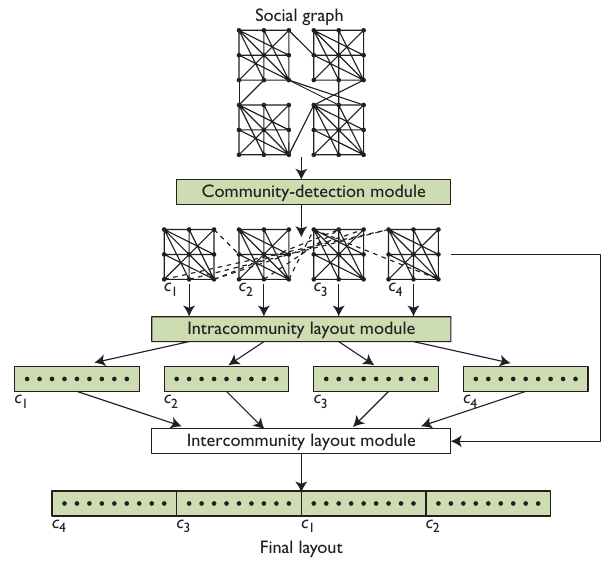
\includegraphics[keepaspectratio,width=0.8\textwidth]{img/06-rel_w/bondhu.png}
        \end{center}
        \caption{Broad steps performed by the bondhu algorithm~\autocite{hoque2012disk}.} 
        \label{bondhu-fig}
    \end{figure}

    The authors propose an incremental placement schema within a block:
    Place the node with the highest degree in the middle of the block, select the node with the heaviest edge connected to the first node and place it next to the first node. 
    After these two placements, a new graph is created, where the two already placed nodes are merged, and their relationships are aggregated. 
    The node with the next heaviest edge is selected and placed alternatingly. The previous two steps are repeated until all nodes are placed within blocks.
    This is done for every community.
    In the final part of the method, the intercommunity layout is derived. 
    Here each community is a vertex, and the edges between those are just the accumulated edges of the underlying graph. 
    After creating the graph, the previous alternating placement schema is applied.
    
    \subsection*{Louvain-like Formation and RCM-based Ordering}
        As a first step, a contraction algorithm that optimizes the modularity or the CPM~\autocite{traag2011narrow, potts1952some} function is executed.
        During the contraction step of the Louvain or the Leiden algorithm~\autocite{traag2019louvain}, it is easy to stop merging when communities reach a certain number of nodes.
        That is, as soon as a community has $\frac{\text{Block Size}}{\text{node size}}$ nodes, then do not consider merging nodes into it anymore.
        This results in block-sized partitions.
        The aggregation step of these algorithms can then be performed as is. 
        Afterward, executing the algorithm in its standard form yields a hierarchy of graphs, similar to the method employed in G-Store.
    
        This can then be used to achieve an ordering of the blocks:
        Uncoarsen the graph by applying the Dewey numbering scheme~\autocite{dewey1894decimal}, employed by ICBL and G-Store.
        Additionally, a heuristic for improving the vertex ordering can be applied layerwise. 
        A recent comprehensive survey of minimum linear arrangement approximation algorithms can be found in~\autocite{barik2020vertex}.
        An appealing option would be to apply the reverse Cuthill-McKee (RCM) algorithm~\autocite{Cuthill1969ReducingTB}, that approximates the solution in $\mathcal{O}(|V| \cdot \text{deg}{V}) = \mathcal{O}(|E|)$. 
        It first finds a peripheral vertex.
        It starts a modified version of the breadth-first search that sorts the nodes by traversal order and degree.
        The quality of the algorithm is highly dependent on the input graph.
        As the input graph is the already approximately ordered graph from the last level, input ordering effects should be mitigated.
        The algorithm compared to other state-of-the-art methods is described by Barik et al.~\autocite{barik2020vertex}.
        
        After the algorithms above are finished, the vertices are laid out in this order to file. 
        The relationships are written to file in the same order by grouping and storing the vertex's outgoing edges and to follow the vertex order.
        The outgoing edges of the vertex stored at the first slot in the vertex file are stored beginning at the first slot of the edge file. 
        The outgoing edges of the second node start right after the edge group of the first node.
        This scheme is motivated by the assumption that traversals in directed graphs follow the edge direction.
        
\chapter{Evaluation Data}
\section*{C. Elegans Frontal Neural Network Dataset}
\begin{table}[H]
	\begin{center}
		 \begin{tabular}[c]{c c c c c c} \toprule
			  & BFS & DFS & Dijkstra & $A^*$  & ALT \\ \midrule 
 			\multirow{2}{*}{Natural}  & 118 & 112 & 113 & 16 & 8 \\ 
 				 & 1025 & 1026 & 1026 & 158 & 67 \\ 
 				&&&&& \\[-0.5em]
 			\multirow{2}{*}{Random}  & 120 & 121 & 118 & 81 & 102 \\ 
 				 & 1036 & 1028 & 1035 & 772 & 940 \\ 
 				&&&&& \\[-0.5em]
 			\multirow{2}{*}{Louvain}  & 74 & 66 & 79 & 10 & 15 \\ 
 				 & 749 & 714 & 647 & 101 & 196 \\ 
 				&&&&& \\[-0.5em]
 			\multirow{2}{*}{G-Store}  & 75 & 89 & 75 & 13 & 24 \\ 
 				 & 581 & 652 & 570 & 149 & 366 \\ 
 				&&&&& \\[-0.5em]
 			\multirow{2}{*}{ICBL}  & 96 & 86 & 66 & 12 & 40 \\ 
 				 & 695 & 734 & 819 & 107 & 349 \\ 
 				&&&&& \\[-0.5em]
 					\end{tabular}  
  	 \end{center}
	 \caption{Comparison of IOs per method, query and record type on the C. elegans dataset with unsorted incidence lists.}
	 \label{ce-uns}
\end{table}

\begin{table}[H]
	\begin{center}
		 \begin{tabular}[c]{c c c c c c} \toprule
			  & BFS & DFS & Dijkstra & $A^*$  & ALT \\ \midrule 
 			\multirow{2}{*}{Natural}  & 114 & 114 & 111 & 11 & 35 \\ 
 				 & 952 & 944 & 952 & 110 & 366 \\ 
 				&&&&& \\[-0.5em]
 			\multirow{2}{*}{Random}  & 122 & 114 & 121 & 71 & 97 \\ 
 				 & 961 & 960 & 957 & 665 & 785 \\ 
 				&&&&& \\[-0.5em]
 			\multirow{2}{*}{Louvain}  & 83 & 82 & 69 & 14 & 17 \\ 
 				 & 222 & 389 & 145 & 60 & 99 \\ 
 				&&&&& \\[-0.5em]
 			\multirow{2}{*}{G-Store}  & 73 & 86 & 75 & 16 & 30 \\ 
 				 & 178 & 280 & 228 & 77 & 168 \\ 
 				&&&&& \\[-0.5em]
 			\multirow{2}{*}{ICBL}  & 84 & 81 & 67 & 12 & 46 \\ 
 				 & 146 & 167 & 355 & 106 & 197 \\ 
 				&&&&& \\[-0.5em]
 					\end{tabular}  
  	 \end{center}
	 \caption{Comparison of IOs per method, query and record type on the C. elegans dataset with sorted incidence lists.}
	 \label{ce-s}
\end{table}

\section*{European Research Email Network Dataset}
\begin{table}[H]
	\begin{center}
		 \begin{tabular}[c]{c c c c c c} \toprule
			  & BFS & DFS & Dijkstra & $A^*$  & ALT \\ \midrule 
 			\multirow{2}{*}{Natural}  & 970 & 972 & 972 & 326 & 774 \\ 
 				 & 39123 & 39114 & 39123 & 22834 & 34759 \\ 
 				&&&&& \\[-0.5em]
 			\multirow{2}{*}{Random}  & 973 & 966 & 971 & 99 & 132 \\ 
 				 & 39105 & 39097 & 39106 & 8389 & 10319 \\ 
 				&&&&& \\[-0.5em]
 			\multirow{2}{*}{Louvain}  & 605 & 638 & 773 & 321 & 400 \\ 
 				 & 27778 & 29728 & 30127 & 28255 & 24875 \\ 
 				&&&&& \\[-0.5em]
 			\multirow{2}{*}{G-Store}  & 685 & 647 & 751 & 206 & 331 \\ 
 				 & 24234 & 28923 & 25016 & 10397 & 14441 \\ 
 				&&&&& \\[-0.5em]
 			\multirow{2}{*}{ICBL}  & 771 & 633 & 585 & 347 & 162 \\ 
 				 & 30453 & 21861 & 25379 & 21617 & 10448 \\ 
 				&&&&& \\[-0.5em]
 					\end{tabular}  
  	 \end{center}
	 \caption{Comparison of IOs per method, query and record type on the email dataset with unsorted incidence lists.}
	 \label{email-uns}
\end{table}

\begin{table}[H]
	\begin{center}
		 \begin{tabular}[c]{c c c c c c} \toprule
			  & BFS & DFS & Dijkstra & $A^*$  & ALT \\ \midrule 
 			\multirow{2}{*}{Natural}  & 952 & 947 & 966 & 316 & 762 \\ 
 				 & 29223 & 29221 & 29225 & 16340 & 25755 \\ 
 				&&&&& \\[-0.5em]
 			\multirow{2}{*}{Random}  & 908 & 949 & 932 & 43 & 72 \\ 
 				 & 29236 & 29231 & 29237 & 4127 & 5432 \\ 
 				&&&&& \\[-0.5em]
 			\multirow{2}{*}{Louvain}  & 629 & 592 & 539 & 407 & 399 \\ 
 				 & 5169 & 8945 & 8247 & 8042 & 4978 \\ 
 				&&&&& \\[-0.5em]
 			\multirow{2}{*}{G-Store}  & 748 & 650 & 549 & 204 & 111 \\ 
 				 & 8024 & 6454 & 6490 & 4488 & 1010 \\ 
 				&&&&& \\[-0.5em]
 			\multirow{2}{*}{ICBL}  & 558 & 733 & 664 & 164 & 268 \\ 
 				 & 4504 & 9007 & 4849 & 6316 & 5776 \\ 
 				&&&&& \\[-0.5em]
 					\end{tabular}  
  	 \end{center}
	 \caption{Comparison of block IOs per method, query and record type on the email dataset with sorted incidence lists.}
	 \label{email-s}
\end{table}

\section*{DBLP Citation Network Dataset}
\begin{table}[H]
	\begin{center}
		 \begin{tabular}[c]{c c c c c c} \toprule
			  & BFS & DFS & Dijkstra & $A^*$  & ALT \\ \midrule 
 			\multirow{2}{*}{Natural}  & 317072 & 317071 & 317071 & 88454 & 239225 \\ 
 				 & 1338193 & 1314632 & 1344250 & 598168 & 1135678 \\ 
 				&&&&& \\[-0.5em]
 			\multirow{2}{*}{Random}  & 317063 & 317064 & 317070 & 2338 & 91026 \\ 
 				 & 1338218 & 1314495 & 1344206 & 20784 & 506800 \\ 
 				&&&&& \\[-0.5em]
 			\multirow{2}{*}{Louvain}  & 209269 & 231464 & 190242 & 27762 & 219532 \\ 
 				 & 1003659 & 906895 & 846871 & 249979 & 723742 \\ 
 				&&&&& \\[-0.5em]
 			\multirow{2}{*}{G-Store}  & 250482 & 187065 & 215604 & 16340 & 97658 \\ 
 				 & 842998 & 972704 & 752748 & 156619 & 409640 \\ 
 				&&&&& \\[-0.5em]
 					\end{tabular}  
  	 \end{center}
	 \caption{Comparison of IOs per method, query and record type on the DBLP dataset with unsorted incidence lists.}
	 \label{dblp-uns}
\end{table}

\begin{table}[H]
	\begin{center}
		 \begin{tabular}[c]{c c c c c c} \toprule
			  & BFS & DFS & Dijkstra & $A^*$  & ALT \\ \midrule 
 			\multirow{2}{*}{Natural}  & 317072 & 317064 & 317076 & 15934 & 242959 \\ 
 				 & 1335990 & 1322882 & 1341846 & 145842 & 1141861 \\ 
 				&&&&& \\[-0.5em]
 			\multirow{2}{*}{Random}  & 317058 & 317065 & 317062 & 2725 & 88404 \\ 
 				 & 1335872 & 1322426 & 1341851 & 23601 & 487566 \\ 
 				&&&&& \\[-0.5em]
 			\multirow{2}{*}{Louvain}  & 190245 & 218779 & 206096 & 32042 & 174006 \\ 
 				 & 495939 & 300461 & 179801 & 65190 & 426641 \\ 
 				&&&&& \\[-0.5em]
 			\multirow{2}{*}{G-Store}  & 187067 & 221947 & 231457 & 19841 & 127806 \\ 
 				 & 486164 & 285141 & 287917 & 87398 & 168100 \\ 
 				&&&&& \\[-0.5em]
 					\end{tabular}  
  	 \end{center}
	 \caption{Comparison of IOs per method, query and record type on the DBLP dataset with sorted incidence lists.}
	 \label{dblp-s}
\end{table}

\section*{Amazon Frequently bought together Dataset}
\begin{table}[H]
	\begin{center}
		 \begin{tabular}[c]{c c c c c c} \toprule
			  & BFS & DFS & Dijkstra & $A^*$  & ALT \\ \midrule 
 			\multirow{2}{*}{Natural}  & 334854 & 334846 & 334854 & 23591 & 206718 \\ 
 				 & 1275141 & 1261562 & 1278263 & 121074 & 859489 \\ 
 				&&&&& \\[-0.5em]
 			\multirow{2}{*}{Random}  & 334844 & 334839 & 334845 & 4630 & 81595 \\ 
 				 & 1274993 & 1261169 & 1278126 & 21735 & 340428 \\ 
 				&&&&& \\[-0.5em]
 			\multirow{2}{*}{Louvain}  & 254490 & 237746 & 267880 & 7217 & 90032 \\ 
 				 & 994592 & 971234 & 1022546 & 33642 & 363483 \\ 
 				&&&&& \\[-0.5em]
 			\multirow{2}{*}{G-Store}  & 217652 & 254487 & 237742 & 17030 & 169893 \\ 
 				 & 969107 & 946004 & 945848 & 88412 & 856992 \\ 
 				&&&&& \\[-0.5em]
 					\end{tabular}  
  	 \end{center}
	 \caption{Comparison of IOs per method, query and record type on the Amazon dataset with unsorted incidence lists.}
	 \label{amazon-uns}
\end{table}

\begin{table}[H]
	\begin{center}
		 \begin{tabular}[c]{c c c c c c} \toprule
			  & BFS & DFS & Dijkstra & $A^*$  & ALT \\ \midrule 
 			\multirow{2}{*}{Natural}  & 334831 & 334831 & 334838 & 29305 & 213728 \\ 
 				 & 1271978 & 1253135 & 1275516 & 148144 & 881883 \\ 
 				&&&&& \\[-0.5em]
 			\multirow{2}{*}{Random}  & 334826 & 334833 & 334829 & 5267 & 105294 \\ 
 				 & 1271472 & 1253034 & 1275273 & 24768 & 446134 \\ 
 				&&&&& \\[-0.5em]
 			\multirow{2}{*}{Louvain}  & 210935 & 194200 & 237722 & 7544 & 105341 \\ 
 				 & 531443 & 184171 & 327139 & 16324 & 97106 \\ 
 				&&&&& \\[-0.5em]
 			\multirow{2}{*}{G-Store}  & 224334 & 254463 & 210939 & 20196 & 186835 \\ 
 				 & 349005 & 395952 & 192827 & 47784 & 418902 \\ 
 				&&&&& \\[-0.5em]
 					\end{tabular}  
  	 \end{center}
	 \caption{Comparison of IOs per method, query and record type on the amazon dataset with sorted incidence lists.}
	 \label{amazon-s}
\end{table}

\section*{YouTube Social Network Dataset}
\begin{table}[H]
	\begin{center}
		 \begin{tabular}[c]{c c c c c c} \toprule
			  & BFS & DFS & Dijkstra & $A^*$  & ALT \\ \midrule 
 			\multirow{2}{*}{Natural}  & 1134885 & 1134874 & 1134887 & 520744 & 626139 \\ 
 				 & 3376451 & 3180208 & 3434910 & 3029489 & 2837347 \\ 
 				&&&&& \\[-0.5em]
 			\multirow{2}{*}{Random}  & 1134878 & 1134879 & 1134885 & 494930 & 900538 \\ 
 				 & 3378223 & 3180625 & 3436253 & 2995538 & 3134437 \\ 
 				&&&&& \\[-0.5em]
 			\multirow{2}{*}{Louvain}  & 624186 & 805764 & 714975 & 130763 & 464393 \\ 
 				 & 2432604 & 2385390 & 2748602 & 1315246 & 1918687 \\ 
 				&&&&& \\[-0.5em]
 			\multirow{2}{*}{G-Store}  & 817115 & 783068 & 749022 & 24225 & 128005 \\ 
 				 & 2431757 & 1780594 & 2679796 & 326708 & 957401 \\ 
 				&&&&& \\[-0.5em]
 					\end{tabular}  
  	 \end{center}
	 \caption{Comparison of IOs per method, query and record type on the C. elegans dataset with unsorted incidence lists.}
	 \label{yt-uns}
\end{table}

\begin{table}[H]
	\begin{center}
		 \begin{tabular}[c]{c c c c c c} \toprule
			  & BFS & DFS & Dijkstra & $A^*$  & ALT \\ \midrule 
 			\multirow{2}{*}{Natural}  & 1134879 & 1134869 & 1134870 & 466807 & 673661 \\ 
 				 & 3369934 & 3274601 & 3427327 & 2760899 & 2877905 \\ 
 				&&&&& \\[-0.5em]
 			\multirow{2}{*}{Random}  & 1134841 & 1134858 & 1134858 & 545467 & 743401 \\ 
 				 & 3372967 & 3274050 & 3428718 & 3193624 & 2932793 \\ 
 				&&&&& \\[-0.5em]
 			\multirow{2}{*}{Louvain}  & 885148 & 760368 & 828413 & 129288 & 439661 \\ 
 				 & 1238579 & 1003650 & 809341 & 308880 & 733981 \\ 
 				&&&&& \\[-0.5em]
 			\multirow{2}{*}{G-Store}  & 771704 & 907899 & 646850 & 21961 & 112100 \\ 
 				 & 550333 & 1055840 & 958365 & 147532 & 326985 \\ 
 				&&&&& \\[-0.5em]
 					\end{tabular}  
  	 \end{center}
	 \caption{Comparison of IOs per method, query and record type on the YouTube dataset with sorted incidence lists.}
	 \label{yt-s}
\end{table}
